    \section{Runtime Verification}
    \textit{Runtime Verification} (RV) is a dynamic analysis method aiming at checking whether a run of the system under scrutiny satisfies a given correctness property.

  \begin{figure}
    \centering
    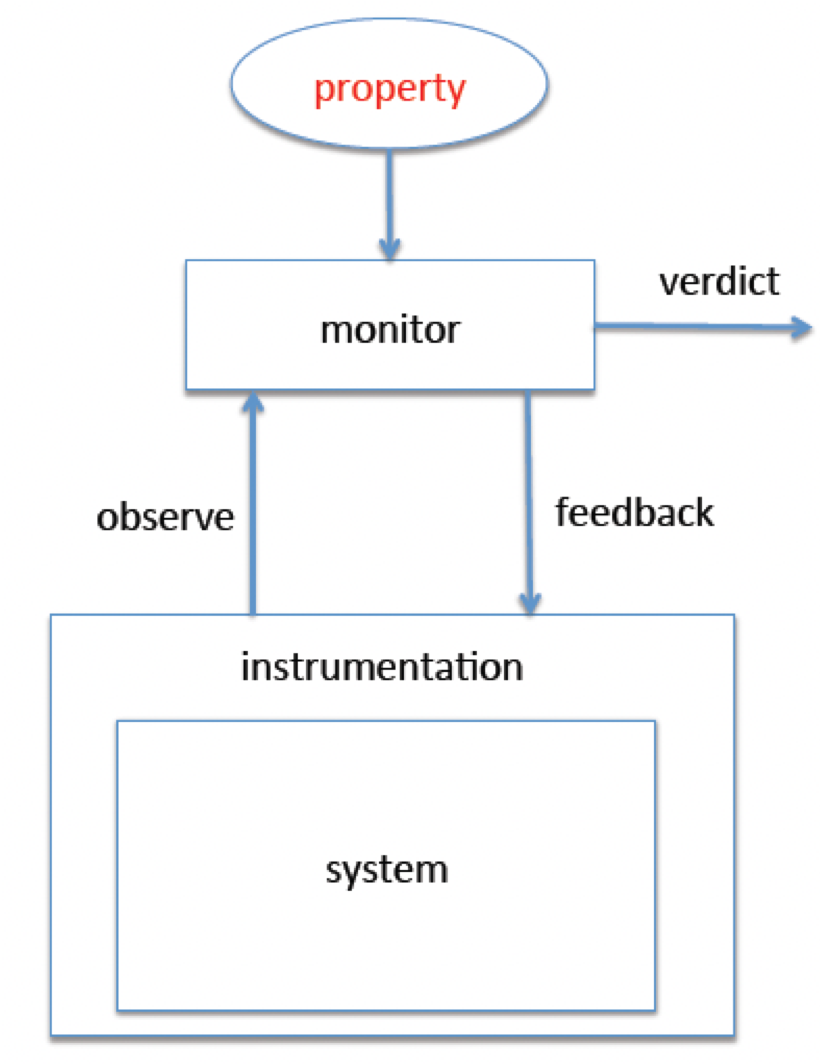
\includegraphics [scale=0.4]{Images/rv.png}
    \caption{An overview of the RV process}
    \label{rv}
\end{figure}

 The components of a RV environment are the system to be checked and a set of properties to be checked against the system execution. Properties can be expressed in a formal specification language, or even as a program in a general-purpose programming language. From a given property, a monitor is generated, i.e., a decision procedure for that property - \textit{monitor synthesis}. The system is instrumented to generate the relevant events to be fed into the monitor - \textit{system instrumentation}. In the next step, the system's execution is analyzed by the monitor - \textit{execution analysis}. The monitor is able to consume the events produced by the running system and, for each consumed event, emits a verdict indicating the status of the property, depending on the event sequence seen so far. Finally, the monitor sends feedback to the system so that more specific corrective actions can be taken (Figure \ref{rv}) ~\cite{rvart}.
 
 
\subsection{Formal Specification of the system behaviour}
There are different formal approaches to describe the expected behaviour of a system. But before presenting some different specification languages, let's start by presenting some general properties of these formalisms. 

\subsubsection{Events}
The behaviour of a system can be analyzed as the way the system changes over time, and this can be done through its observation. To abstract these observations we will use \textit{Events} - discrete atomic entities that represent \textit{actions} or \textit{state changes} made by the system. 
The system's observable events of interest is called its \textit{alphabet}. The choice of events is part of the specification and will determine the available information about the system and about which properties can be described.

\subsubsection{Traces}
A \textit{trace} is a sequence of events and abstracts the behaviour of a single run of the system. Obviously, an observable trace must be finite, but it is sometimes useful to think about the possible infinite behaviours of a system. Therefore, a trace can be viewed as a finite prefix of the infinite behaviour.

\subsubsection{Properties and Specifications}
The abstraction of a property can be described as a set of traces and its specification is a concrete (textual) object that denotes this set of traces.
As there are many specifications languages, one can have many specifications for a single property, but a property is unique and independent of the specification language. If the specification language is ambiguous, then the specific property may not be clear. Dealing with such ambiguities is a common issue in the specification process ~\cite{rv2}.


\subsection{Different language specifications}
This section presents a brief description of the main specification languages for RV, as well as some of their general features.

A RV specification language can be \textit{Executable} if the specification is directly executable and therefore more low-level, or \textit{Declarative} in which an executable object (monitor) is generated from the specification. Also, some specification languages are more suited to specify sets of finite traces whereas others are more suited to specify infinite traces. A specification may also capture \textit{good} or \textit{bad} behaviour. A match against a good behaviour specification represents \textit{validation} of the desired property, whereas a match a bad behaviour specification represents \textit{violation} of that property ~\cite{rv2}.

\subsubsection{Regular Expressions}
Regular Expressions are a commonly used formalism in Computer Science for describing sets of strings, but can also be used in RV to describe traces of events, where the atoms are not characters but events. The regular expression matches if any \textit{suffix} of the trace matches the expression - \textit{suffix-matching} - to attest the validation or violation of the property (e.g., in the work of TraceMatches) ~\cite{rvart}.

\subsubsection{Finite State Machines}
Finite State machines have the same expressive power of Regular Expressions but have the advantage of being directly executable, in opposition to regular expressions and temporal logic, since both require \textit{monitor synthesis} to produce a monitor, which is usually described as some form of state machine. 

\vspace{5mm}

The formalisms of \textbf{Linear Temporal Logic} and \textbf{Context Free Grammars} can also be used for specifications in RV, but since they are not the main focus of the present work they will not be further approached. 
